\documentclass[12pt]{article}
\usepackage{times}
\usepackage{amsmath}
\usepackage{amssymb}
\usepackage[pdftex]{graphicx}
\usepackage{epstopdf}
\usepackage{booktabs}
\usepackage{array}
\usepackage{ITC}

\title{\Large \vspace{-0.5in}
\MakeUppercase{Performance Evaluation of Monocular and Stereo Vision for Autonomous UAV Collision Avoidance in Disaster Response Environments}}
\author{Clinton Imaro\\
    \normalsize Center for Equitable AI and Machine Learning Systems\\
    \normalsize Department of Computer Science\\
    \normalsize Morgan State University\\
    \normalsize Baltimore, MD, USA\\
    \normalsize clima1@morgan.edu\\[6pt]
    \normalsize Faculty Advisor: Peter Taiwo\\
    \normalsize Center for Equitable AI and Machine Learning Systems\\
    \normalsize Department of Electrical and Computer Engineering\\
    \normalsize Morgan State University\\
    \normalsize Baltimore, MD, USA\\
    \normalsize peter.taiwo@morgan.edu}
\date{}

\begin{document}

\maketitle

\section{\MakeUppercase{Abstract}}

\noindent
Autonomous UAVs in disaster response face dual threats from environmental hazards and physical obstacles. This paper presents a vision-integrated navigation system combining disaster awareness with real-time collision avoidance. A PPO navigation policy trained with CNN-based hazard awareness is reused with depth-derived obstacle-risk maps to evaluate whether a single monocular camera can support practical obstacle avoidance compared with a heavier stereo configuration. Stereo depth is estimated with OpenCV StereoSGBM, while monocular depth is generated from the left image using MiDaS Small. Both perception modes are converted to a common risk-map interface and evaluated against simulator ground truth using success rate, collision rate, path efficiency, obstacle clearance, latency, and robustness under perception degradation. Raw PPO transfer is unsafe, producing 0.000 success and 0.600 collision rate in clean evaluation. With an evaluation-time safety shield, collision rate falls to 0.000 for both sensing modes. Monocular PPO+shield reaches 0.956 clean success at 40.84 ms total inference latency, while stereo reaches 0.808 success at 12.26 ms. The results identify a clear trade-off: stereo is faster, but monocular sensing is more robust in several degraded conditions.

\section{\MakeUppercase{Key Words}}

\noindent
UAV navigation; collision avoidance; monocular depth; stereo vision; reinforcement learning.

\section{\MakeUppercase{Introduction}}

\noindent
Autonomous UAVs are useful in disaster response because they can inspect damaged areas, collect imagery, and support situational awareness without exposing human responders to unstable structures. In practice, the same environment that motivates UAV deployment also creates difficult navigation conditions. A vehicle may need to avoid buildings, poles, debris, smoke-obscured structures, and damaged infrastructure while operating with limited onboard compute and payload capacity. For small UAVs, stereo cameras provide geometric depth but add hardware, calibration, synchronization, and processing requirements. A monocular camera is lighter and simpler, but monocular depth is generally relative rather than metric and can be less reliable near unfamiliar structures.

This paper studies that trade-off directly. The objective is not to claim that monocular depth is a complete substitute for stereo geometry in all conditions. Instead, the goal is to measure whether a monocular depth model can produce a navigation-usable obstacle-risk interface and how that interface compares with a stereo baseline when both are used by the same UAV collision-avoidance controller.

The work builds on a frozen PPO navigation policy originally trained for hazard-aware grid navigation. Stereo and monocular depth outputs are converted into a common $50 \times 50$ risk-map representation and inserted into the same four-channel PPO observation format. No PPO retraining or architecture change is used in the main evaluation. This constraint is intentional: it isolates the effect of the perception interface and safety logic rather than introducing a new policy for each sensor mode.

The main contributions are:

\begin{itemize}
\item A stereo-to-risk baseline using UAVStereo residential imagery and OpenCV StereoSGBM.
\item A monocular-to-risk baseline using MiDaS Small on the left camera image only.
\item A shared risk-map interface that allows both perception modes to drive the same PPO navigation policy.
\item A PPO+shield controller that preserves the frozen policy while enforcing local collision-safety checks.
\item A clean-condition, robustness, and hazard-density evaluation comparing success, collision rate, path efficiency, clearance, latency, and failure modes.
\end{itemize}

\section{\MakeUppercase{Related Work}}

\noindent
Stereo matching is a classical approach for dense depth estimation from rectified image pairs. Semi-global matching estimates disparity by combining local matching costs with smoothness penalties over multiple path directions, providing a practical balance between local block matching and fully global optimization \cite{hirschmuller2008sgm}. OpenCV StereoSGBM is a widely used implementation of this family of methods and provides an accessible stereo baseline for robotics experiments \cite{opencvsgbm}.

Monocular depth estimation estimates scene structure from a single image. MiDaS and related dense prediction methods are trained across mixed datasets to improve cross-dataset generalization, but they typically output relative depth that must be scaled or calibrated before being interpreted as metric distance \cite{ranftl2022midas}. Dense Prediction Transformers further improved monocular dense prediction by using transformer backbones for global image context \cite{ranftl2021dpt}. For a small UAV, monocular depth has an attractive hardware profile, but its safety value depends on whether relative depth is stable enough for obstacle avoidance.

UAVStereo provides stereo imagery and disparity references for low-altitude UAV scenarios, addressing the shortage of stereo datasets that resemble UAV viewpoints rather than road-vehicle perspectives \cite{uavstereo2023}. This work uses the residential sequence from UAVStereo as the perception data source. The navigation controller follows prior work on PPO, which optimizes a clipped policy objective for stable policy updates \cite{schulman2017ppo}. The experiments also draw on disaster-aware hazard mapping from aerial imagery, where visual classifiers such as those trained on AIDER-style datasets can support risk-aware UAV planning \cite{aider2020}.

\section{\MakeUppercase{System Design and Methods}}

\subsection{Stereo Depth Baseline}

\noindent
The stereo baseline uses synchronized left and right UAVStereo residential frames. For each rectified pair, OpenCV StereoSGBM estimates a dense disparity image $d(u,v)$ over pixel coordinates $(u,v)$. A depth proxy is computed as
\begin{equation}
Z_s(u,v)=\frac{fB}{d(u,v)+\epsilon}.
\end{equation}
Here $Z_s$ is the stereo depth proxy, $f$ is focal length in pixels, $B$ is stereo baseline, and $\epsilon$ prevents division by zero in invalid or near-zero disparity regions. The implementation uses the UAVStereo residential baseline sequence `ZM-Baseline-25' and processes frames 0010 through 0150.

The obstacle decision is defined with a fixed collision threshold:
\begin{equation}
O_s(u,v)=
\begin{cases}
1, & Z_s(u,v) < Z_c,\\
0, & Z_s(u,v) \geq Z_c,
\end{cases}
\end{equation}
where $Z_c=2.5$ m is the collision-proxy threshold. A normalized risk value is then computed as
\begin{equation}
R_s(u,v)=\min\left(1,\frac{Z_c}{Z_s(u,v)+\epsilon}\right).
\end{equation}
The risk map is later resized or pooled into the navigation grid representation.

\subsection{Monocular Depth Baseline}

\noindent
The monocular baseline uses only the left UAVStereo image. MiDaS Small produces a relative inverse-depth output $M(u,v)$. Since monocular depth is not directly metric, the output is calibrated against the available stereo/disparity reference on shared valid pixels. The calibrated monocular depth proxy is represented as
\begin{equation}
Z_m(u,v)=\alpha \hat{Z}_m(u,v),
\end{equation}
where $\hat{Z}_m$ is the raw monocular depth proxy and $\alpha$ is a scale factor estimated from the shared frame set. The calibrated scale factor was $0.4413$. The same obstacle and risk-map definitions are then applied:
\begin{equation}
O_m(u,v)=\mathbb{1}[Z_m(u,v)<Z_c],
\end{equation}
\begin{equation}
R_m(u,v)=\min\left(1,\frac{Z_c}{Z_m(u,v)+\epsilon}\right).
\end{equation}
This ensures that stereo and monocular perception produce the same downstream interface: depth proxy, obstacle mask, risk map, collision proxy, and per-frame metrics.

\subsection{Sensor Alignment}

\noindent
Stereo and monocular outputs are aligned by frame ID, resolution, risk range, and obstacle-mask format. Risk maps are bounded to $[0,1]$ and obstacle maps are binary. For each shared frame, risk-map error is measured by
\begin{equation}
\text{MAE}_{R}=\frac{1}{N}\sum_{i=1}^{N}|R_s(i)-R_m(i)|
\end{equation}
and
\begin{equation}
\text{RMSE}_{R}=\sqrt{\frac{1}{N}\sum_{i=1}^{N}(R_s(i)-R_m(i))^2}.
\end{equation}
Obstacle-map agreement is measured by intersection-over-union:
\begin{equation}
\text{IoU}=\frac{|O_s \cap O_m|}{|O_s \cup O_m|}.
\end{equation}
These metrics do not assume that monocular depth equals stereo depth. They verify that both outputs can be compared through a common safety interface.

\subsection{Navigation Input Adapter}

\noindent
The PPO policy expects an observation tensor $X_t \in \mathbb{R}^{50 \times 50 \times 4}$. For both sensing modes the input channels are:

\begin{equation}
X_t=[R, C, D_u, D_g].
\end{equation}
Here $R$ is the selected perception risk map, $C$ is a known-map confidence mask, $D_u$ is a UAV-position distance field, and $D_g$ is a goal-distance field. This adapter preserves the original PPO input shape and the eight-action movement space. The policy is loaded from the existing checkpoint and used only for deterministic inference.

\subsection{Safety Shield}

\noindent
Initial navigation tests showed that raw PPO transfer from hazard maps to depth-derived obstacle maps was unsafe. To address this without retraining, a safety shield was added at evaluation time. The PPO policy proposes action $a_t^{ppo}$. The shield evaluates available actions using local lookahead, obstacle risk, hazard risk, goal progress, and loop penalty. The selected action is
\begin{equation}
a_t=\arg\min_{a\in A}\left(w_r Q_r(a)-w_p Q_p(a)+w_l Q_l(a)\right),
\end{equation}
when the PPO action is unsafe; otherwise $a_t=a_t^{ppo}$. In this expression, $Q_r$ is predicted local risk, $Q_p$ is progress toward the goal, $Q_l$ penalizes repeated-position loops, and $w_r$, $w_p$, and $w_l$ are the configured weights. The experiments use three-step lookahead, collision risk threshold $0.95$, shield caution threshold $0.50$, hazard threshold $0.70$, risk penalty weight $20.0$, progress weight $5.0$, and loop penalty weight $3.0$.

\section{\MakeUppercase{Experimental Setup}}

\noindent
The perception experiments use UAVStereo residential frames 0010 through 0150 from sequence `ZM-Baseline-25'. The stereo baseline uses OpenCV StereoSGBM. The monocular baseline uses Intel MiDaS Small with the left camera image only. Both pipelines generate depth proxy images, obstacle masks, risk maps, visual montages, and CSV metrics.

Navigation experiments use five locked evaluation scenarios derived from the aligned risk maps: Baseline Open, Dense Corridor, Obstacle Cluster, Lateral Maneuver, and Stress Density. Each scenario specifies a frame ID, stereo and monocular risk-map paths, a $50 \times 50$ grid, fixed start and goal cells, and a collision threshold. The PPO checkpoint is reused across all experiments. No training updates are performed during Weeks 4 through 8 evaluation.

The main clean-condition evaluation contains 1,000 episodes: 250 episodes for raw PPO stereo, raw PPO monocular, PPO+shield stereo, and PPO+shield monocular. Robustness evaluation contains 8,000 episodes across four perturbation types, four severity levels, two sensing modes, and 250 episodes per condition. The hazard-density ablation contains 2,000 episodes across two sensing modes, four hazard-density levels, and 250 episodes per condition.

\section{\MakeUppercase{Numerical Results}}

\subsection{Perception Baselines}

\noindent
Table~\ref{tab:perception} summarizes the stereo and monocular perception baselines. StereoSGBM is faster and produces a denser obstacle estimate on the selected UAVStereo frames. MiDaS Small is slower and produces a sparser obstacle estimate after scale calibration. The monocular baseline remains useful because it provides the same obstacle/risk-map interface with a single camera.

\begin{table}[htbp]
\centering
\caption{Perception Baseline Metrics}
\label{tab:perception}
\begin{tabular}{lcc}
\toprule
Metric & StereoSGBM & MiDaS Small \\
\midrule
Frames & 15 & 15 \\
Disparity MAE (px) & 42.68 & 78.44 \\
Disparity RMSE (px) & 46.64 & 85.80 \\
Valid estimate fraction & 0.665 & 0.117 \\
Obstacle fraction & 0.665 & 0.117 \\
Center alert fraction & 0.836 & 0.069 \\
Inference latency (ms) & 11.87 & 17.53 \\
\bottomrule
\end{tabular}
\end{table}

The alignment experiment confirmed structural comparability but not numerical equivalence. The average risk MAE was 0.710, risk RMSE was 0.993, binary obstacle agreement was 0.254, and obstacle IoU was 0.052. The average aligned depth MAE was 0.042 m over the valid overlap, but valid overlap was only 0.036. These values show that monocular and stereo risk maps can be evaluated through the same interface, while also showing that monocular risk should not be treated as a metric stereo replacement.

\begin{figure}[htbp]
\centering
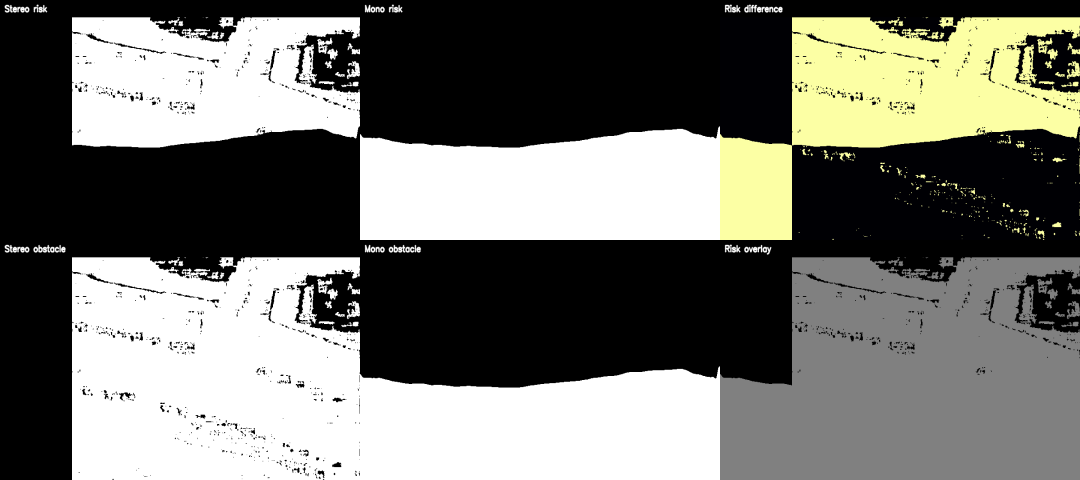
\includegraphics[width=5.75in]{figures/week03_alignment_montage}
\caption{Mono-vs-stereo alignment example showing stereo risk, monocular risk, absolute difference, and obstacle-mask comparison for a locked evaluation frame.}
\label{fig:alignment}
\end{figure}

\subsection{Navigation Integration}

\noindent
Raw PPO integration was first tested without a safety shield. Across 50 episodes, stereo and monocular modes both produced 0.0 success rate and 0.600 collision rate. This result shows that input adaptation alone is insufficient. The PPO checkpoint can execute the navigation loop, but the policy is not safe when depth-derived risk maps are substituted for the original hazard-map distribution.

The shielded-controller evaluation changed the result substantially. In 50 raw PPO and 50 PPO+shield episodes, collision rate fell from 0.600 to 0.000 for both sensing modes. Monocular PPO+shield reached the goal in all 25 shielded episodes. Stereo PPO+shield reached the goal in 22 of 25 shielded episodes and timed out without collision in the remaining 3 episodes.

\subsection{Clean-Condition Performance}

\noindent
Table~\ref{tab:clean} reports the 1,000-episode clean-condition evaluation. Raw PPO is retained as an ablation baseline, not as the final controller. PPO+shield is the deployable controller evaluated in the rest of the paper.

\begin{table}[htbp]
\centering
\caption{Clean-Condition Navigation Results}
\label{tab:clean}
\begin{tabular}{llccccc}
\toprule
Controller & Mode & Runs & Success & Collision & Path Eff. & Latency ms \\
\midrule
Raw PPO & Stereo & 250 & 0.000 & 0.600 & 0.000 & 11.40 \\
Raw PPO & Mono & 250 & 0.000 & 0.600 & 0.000 & 39.99 \\
PPO+shield & Stereo & 250 & 0.808 & 0.000 & 0.641 & 12.26 \\
PPO+shield & Mono & 250 & 0.956 & 0.000 & 0.760 & 40.84 \\
\bottomrule
\end{tabular}
\end{table}

The shield improves success rate by 0.808 for stereo and 0.956 for monocular, while reducing collision rate by 0.600 for both modes. The shield adds approximately 0.82 ms of decision latency. The dominant latency difference is perception: stereo total latency is 12.26 ms with PPO+shield, while monocular total latency is 40.84 ms.

\begin{figure}[htbp]
\centering
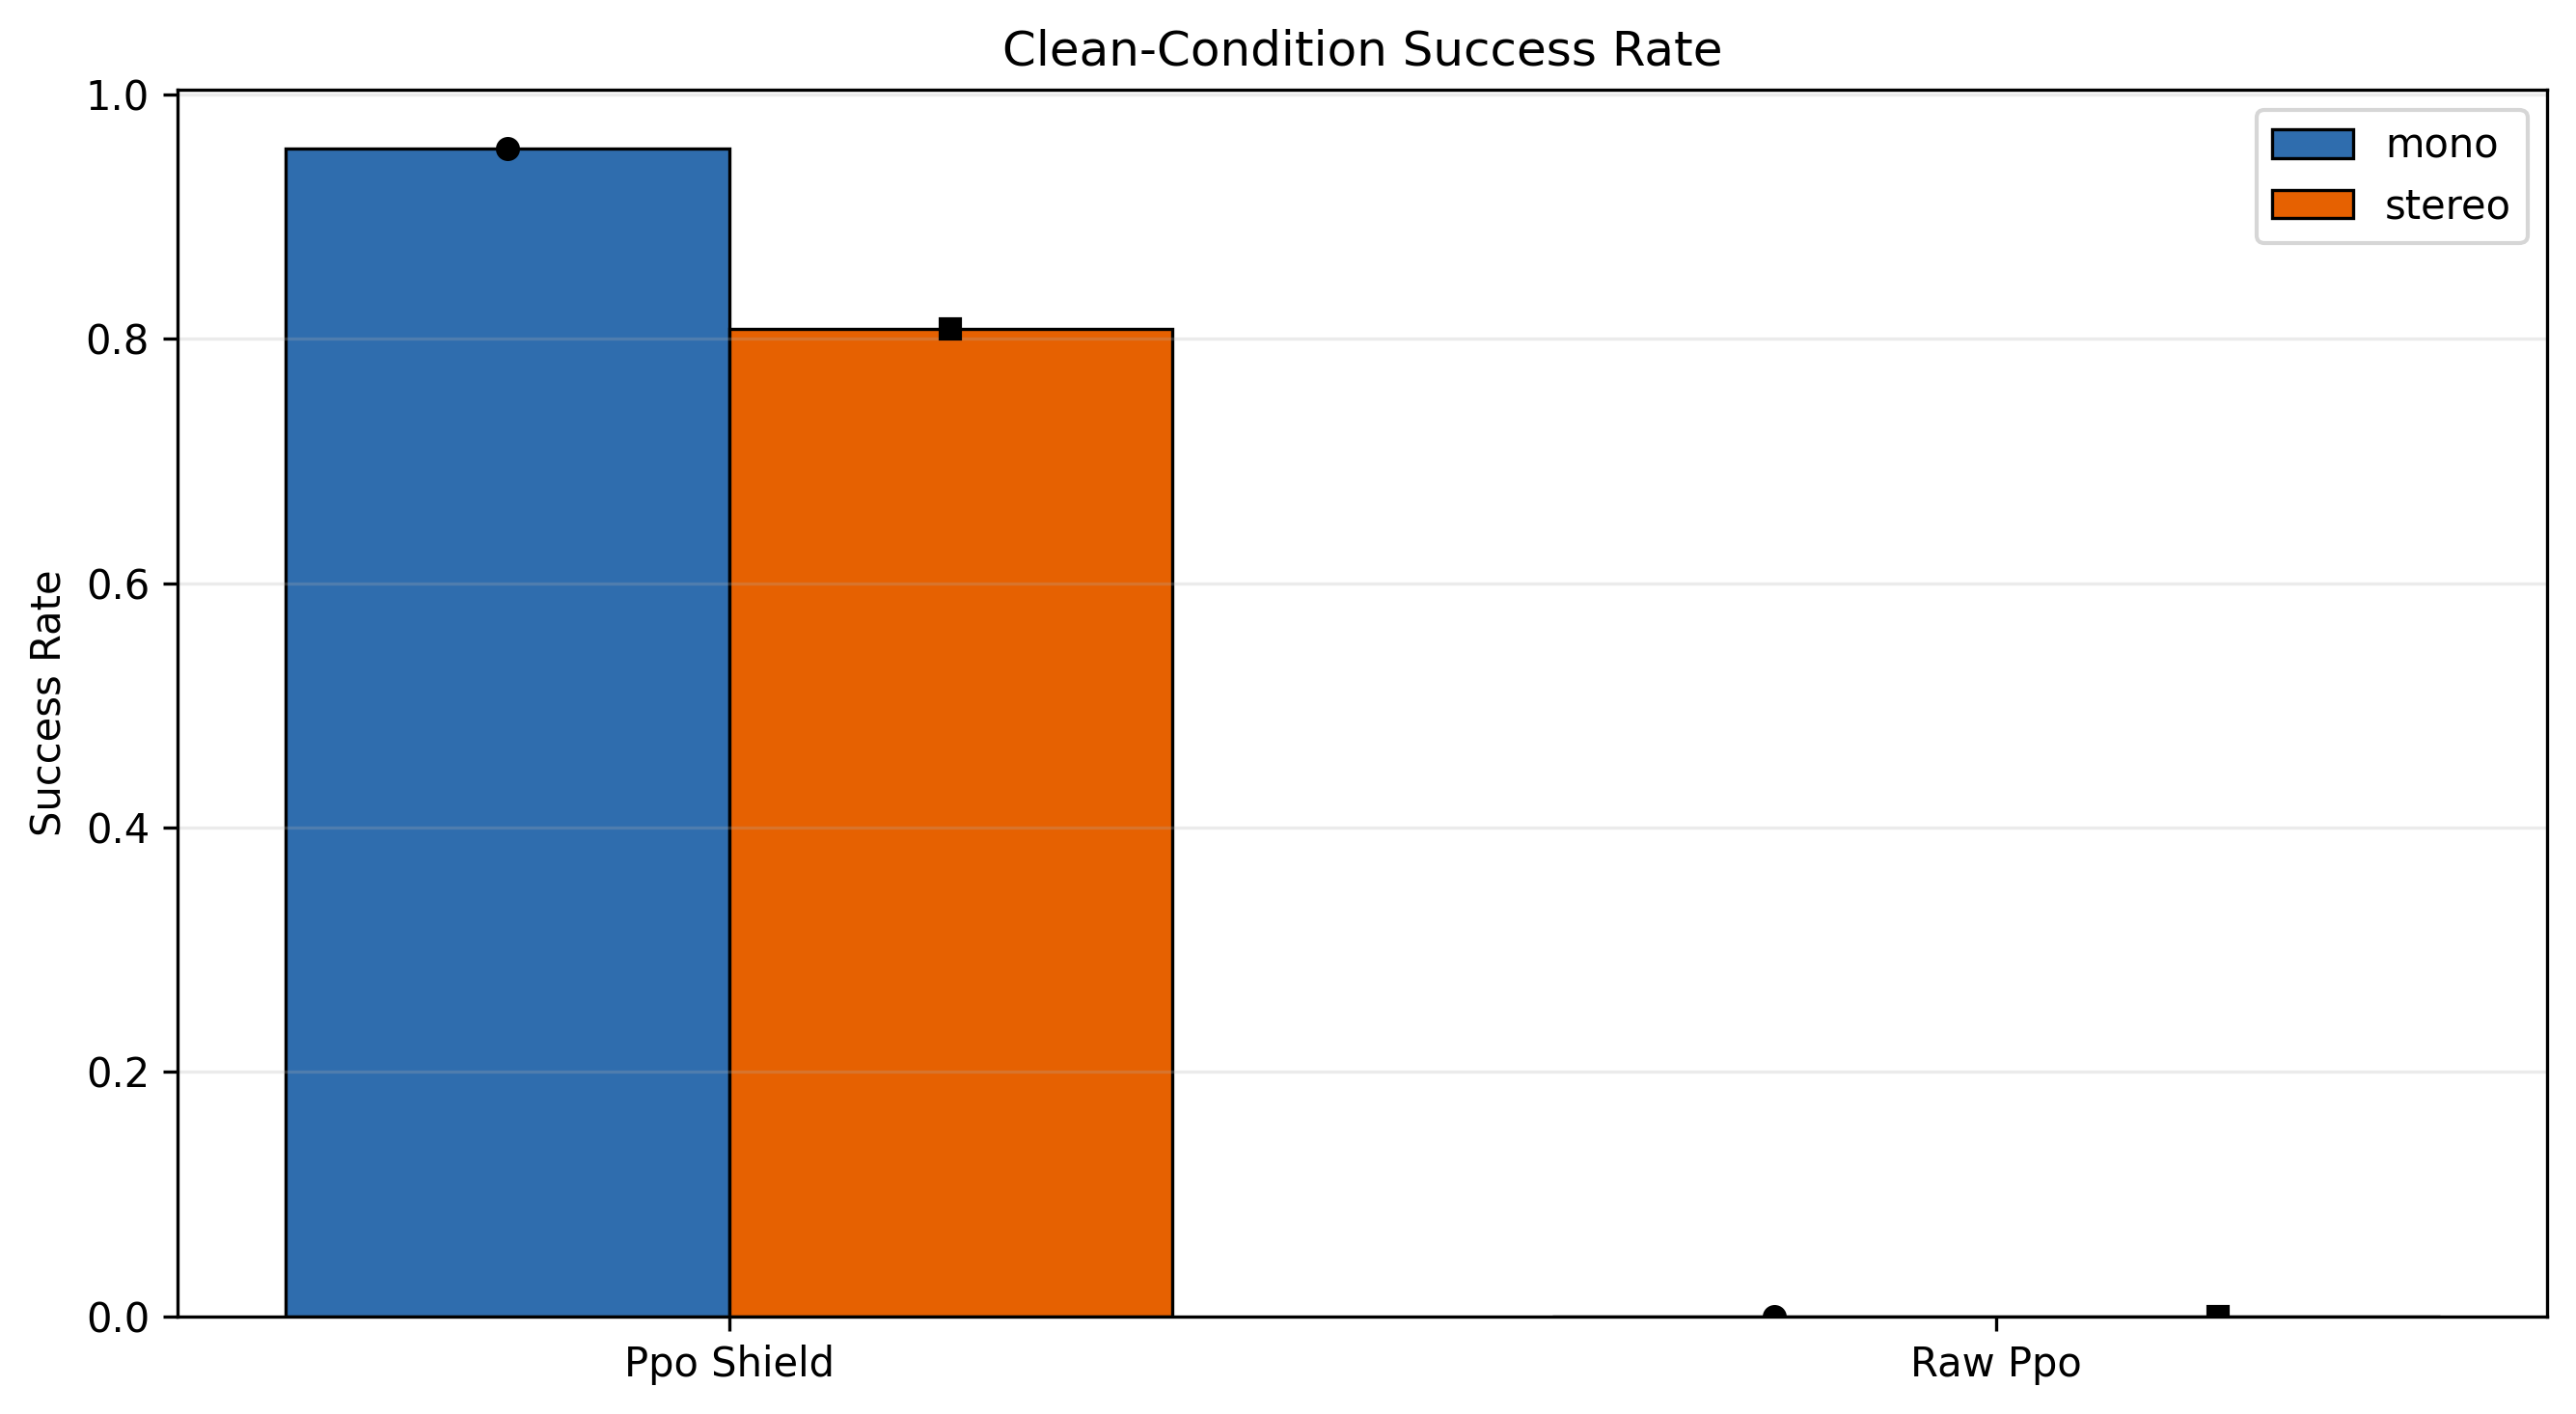
\includegraphics[width=5.75in]{figures/week08_clean_success_rate}
\caption{Clean-condition success rate for raw PPO and PPO+shield under stereo and monocular perception.}
\label{fig:clean_success}
\end{figure}

\begin{figure}[htbp]
\centering
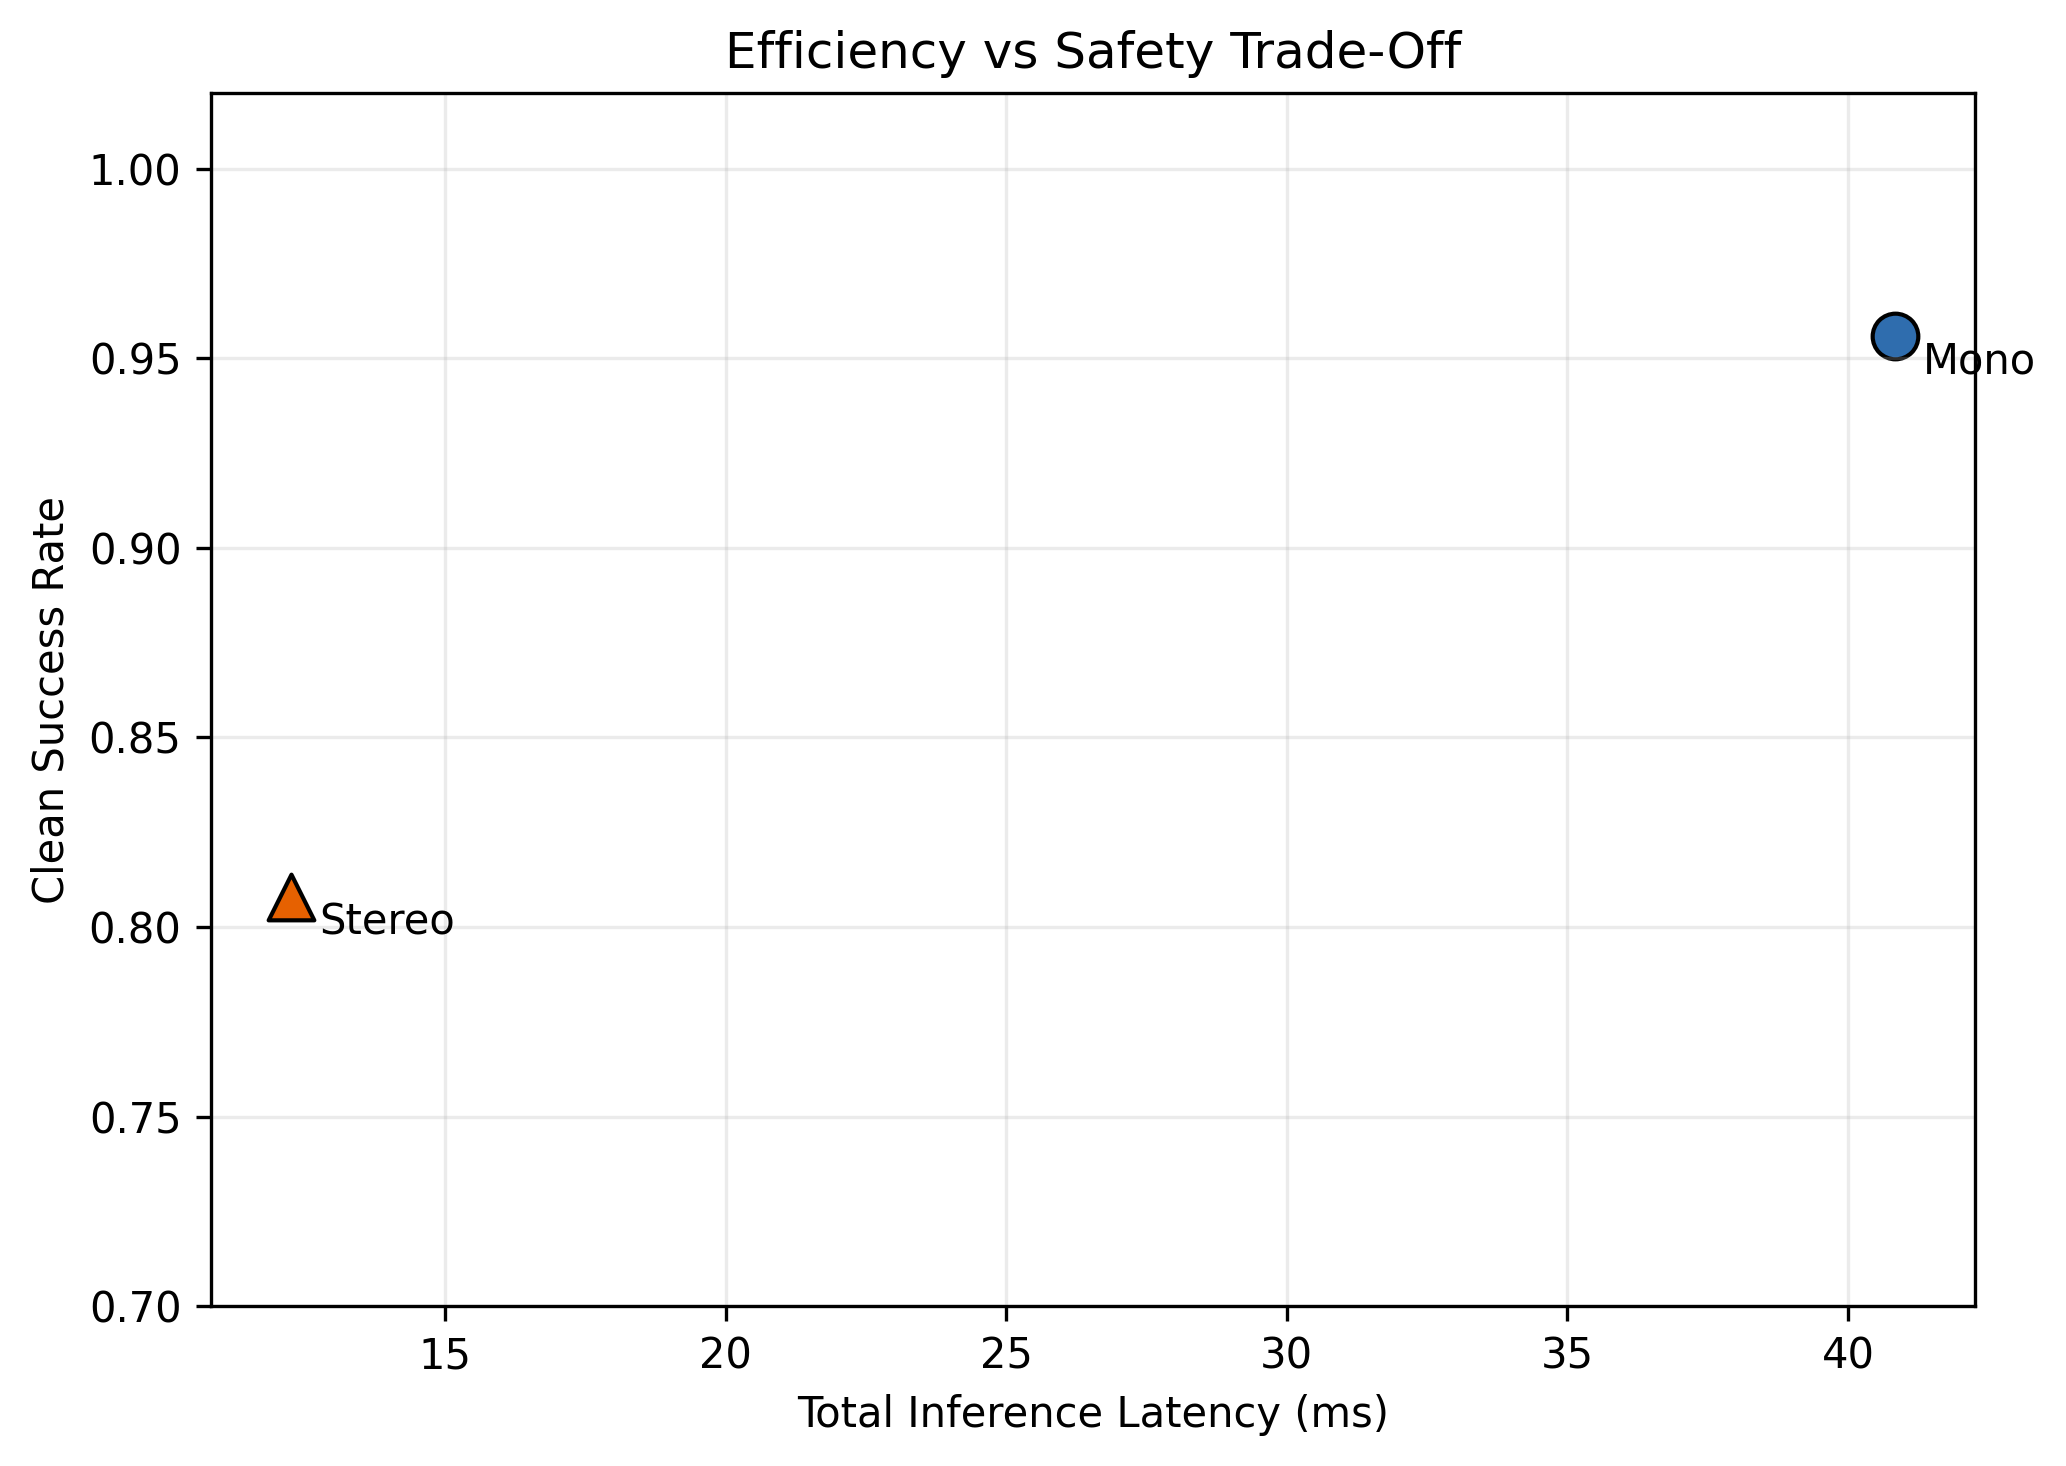
\includegraphics[width=5.75in]{figures/week08_latency_success_tradeoff}
\caption{Latency-success trade-off. Stereo is faster, while monocular achieves higher clean-condition success under the PPO+shield controller.}
\label{fig:latency_tradeoff}
\end{figure}

\subsection{Robustness Under Perception Degradation}

\noindent
Table~\ref{tab:degradation} summarizes worst-case success drops for each perturbation type relative to the clean PPO+shield baseline. Depth noise caused the smallest degradation for both modes. Reduced resolution and blur produced the largest monocular success drops. Partial occlusion was the dominant stereo failure mode.

\begin{table}[htbp]
\centering
\caption{Worst-Case Perception Degradation}
\label{tab:degradation}
\begin{tabular}{llccc}
\toprule
Mode & Perturbation & Worst Sev. & Worst Success & Drop \\
\midrule
Mono & Depth noise & Extreme & 0.908 & 0.048 \\
Mono & Image blur & Extreme & 0.728 & 0.228 \\
Mono & Reduced resolution & Extreme & 0.724 & 0.232 \\
Mono & Partial occlusion & Extreme & 0.832 & 0.124 \\
Stereo & Depth noise & Extreme & 0.764 & 0.044 \\
Stereo & Image blur & High & 0.756 & 0.052 \\
Stereo & Reduced resolution & High & 0.680 & 0.128 \\
Stereo & Partial occlusion & Extreme & 0.404 & 0.404 \\
\bottomrule
\end{tabular}
\end{table}

Partial occlusion also increased stereo collision rate by 0.508 at extreme severity. This occurs because the perturbed risk map can hide obstacle evidence from the controller while physical collision is still checked against the unperturbed obstacle map. Monocular also degrades under occlusion, but the worst success drop is smaller at 0.124.

\begin{figure}[htbp]
\centering
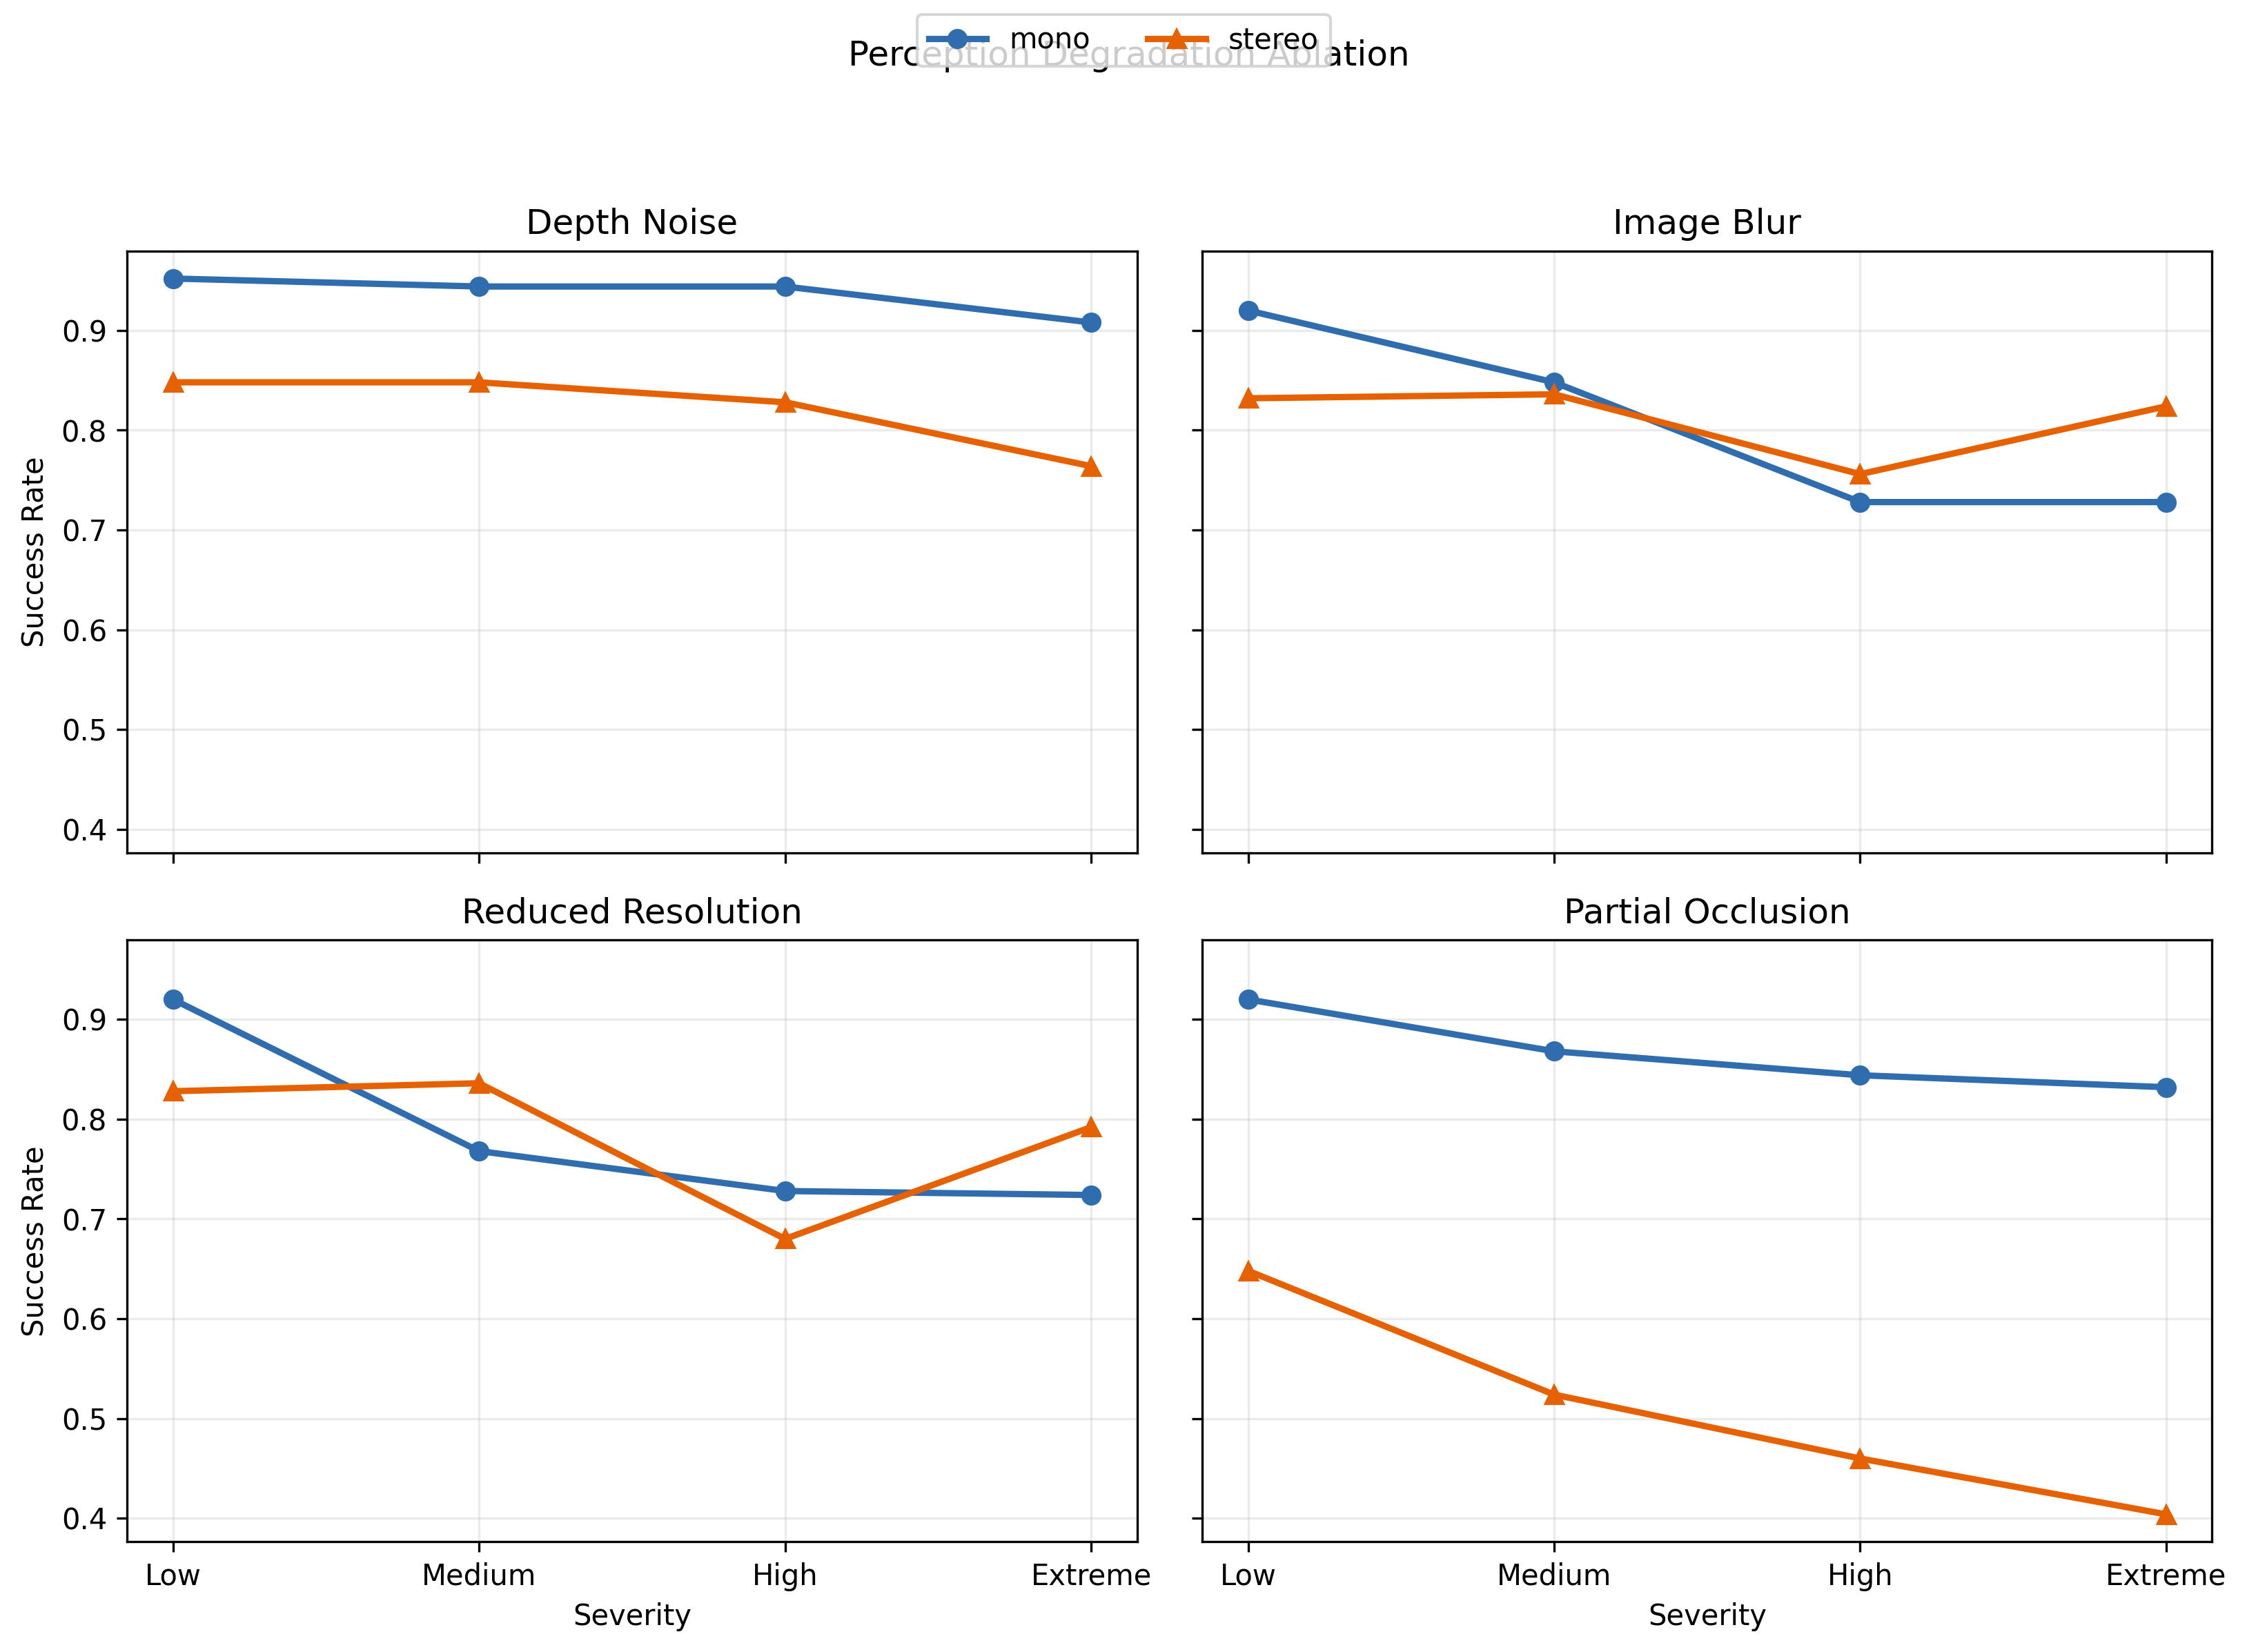
\includegraphics[width=5.75in]{figures/week08_perception_degradation_success}
\caption{Success-rate degradation under controlled depth noise, blur, reduced resolution, and partial occlusion.}
\label{fig:degradation}
\end{figure}

\subsection{Hazard-Density Ablation}

\noindent
Table~\ref{tab:hazard_density} reports the hazard-density ablation. Collision remains 0.000 because physical collision is still evaluated from structural obstacle risk and the safety shield remains active. Increasing hazard density mainly increases timeouts and shield workload.

\begin{table}[htbp]
\centering
\caption{Hazard-Density Ablation with PPO+shield}
\label{tab:hazard_density}
\begin{tabular}{llcccc}
\toprule
Mode & Density & Success & Collision & Exposure & Interventions \\
\midrule
Mono & None & 1.000 & 0.000 & 0.000 & 13.16 \\
Mono & Low & 1.000 & 0.000 & 0.000 & 13.22 \\
Mono & Moderate & 0.952 & 0.000 & 0.032 & 20.64 \\
Mono & High & 0.772 & 0.000 & 0.196 & 47.40 \\
Stereo & None & 0.920 & 0.000 & 0.000 & 31.44 \\
Stereo & Low & 0.908 & 0.000 & 0.000 & 33.34 \\
Stereo & Moderate & 0.740 & 0.000 & 0.032 & 58.97 \\
Stereo & High & 0.436 & 0.000 & 0.396 & 105.93 \\
\bottomrule
\end{tabular}
\end{table}

Under high hazard density, monocular success is 0.772 and stereo success is 0.436. Stereo requires more shield interventions as hazard density increases, reaching an average of 105.93 interventions per episode at high density. The result indicates that the stereo configuration remains computationally faster but is more sensitive to hazard overlays and occlusion in the current risk-map interface.

\section{\MakeUppercase{Discussion}}

\noindent
The experiments support three conclusions. First, raw PPO should not be presented as a safe collision-avoidance controller in this setting. It is useful as an ablation baseline because it shows that simply inserting depth-derived risk maps into the pretrained policy does not solve collision avoidance. The safety shield is necessary to convert the frozen policy into a reliable controller under the tested conditions.

Second, the monocular and stereo pipelines produce different safety trade-offs. Stereo is substantially faster, with 12.26 ms total PPO+shield inference latency compared with 40.84 ms for monocular. This speed advantage matters for onboard telemetry and control loops. However, monocular PPO+shield gives higher clean success in the locked benchmark, 0.956 compared with 0.808 for stereo, and is less severely affected by partial occlusion in the robustness experiment.

Third, the perception metrics explain why the navigation results should be interpreted carefully. MiDaS Small does not match stereo disparity numerically on the selected UAVStereo frames. The low obstacle IoU and negative risk correlation show that the two sensing modes often emphasize different risk regions. The navigation result is therefore not evidence that monocular depth is geometrically equivalent to stereo. It is evidence that a calibrated monocular risk map can support the same collision-avoidance interface and, with a safety shield, can perform competitively in controlled UAVStereo-derived navigation scenarios.

The main limitations are also clear. The navigation episodes are controlled route variants over locked maps, not real flight tests. Perturbations are applied at the perception-interface level rather than by collecting new degraded flight imagery. Minimum obstacle distance is measured in grid-cell clearance from high-risk obstacle cells, not in physical meters. Finally, the controller is PPO+shield rather than raw PPO, so the safety layer must be included in any deployment interpretation.

\section{\MakeUppercase{Conclusions}}

\noindent
This paper evaluated monocular and stereo vision for UAV collision avoidance in disaster-response navigation. StereoSGBM and MiDaS Small were implemented as perception baselines and converted into a shared depth-derived obstacle-risk interface. The shared interface allowed both sensing modes to drive the same frozen PPO navigation policy without architecture changes or retraining.

The experiments show that raw PPO transfer is unsafe, with 0.000 success rate and 0.600 collision rate in clean evaluation. A three-step safety shield reduces clean collision rate to 0.000 for both sensing modes and enables successful navigation under the same policy. In clean conditions, monocular PPO+shield reaches 0.956 success at 40.84 ms total inference latency, while stereo PPO+shield reaches 0.808 success at 12.26 ms. Robustness testing shows that stereo is faster but more vulnerable to partial occlusion, while monocular is slower but more stable under several degraded conditions.

Future work should evaluate the controller on larger UAVStereo scene sets, add real degraded imagery instead of perception-interface perturbations, and test retrained policies that explicitly learn from depth-derived obstacle maps. A hardware deployment should also measure end-to-end camera, inference, telemetry, and control latency on embedded UAV compute.

\section{\MakeUppercase{Acknowledgments}}

\noindent
This work was supported by the Center for Equitable AI and Machine Learning Systems at Morgan State University. The author thanks Peter Taiwo for research supervision and technical feedback.

\bibliographystyle{ieeetr}
\bibliography{references}

\end{document}
